\documentclass{beamer}

\usepackage[utf8]{inputenc}

\usepackage{default}
\usepackage{hyperref}
\usepackage{graphicx}
\usepackage{listings}
\usepackage{tikz}
\usepackage{array}

\newcommand*{\email}[1]{
	\href{mailto:#1}{#1}
}

\title{Approaches to apply Symbolic Execution in non-sequential applications}
\author{Savu Victor-Gabriel}
\institute{Technische Universität München, \email{victorsavu3@gmail.com}}

\definecolor{White}{RGB}{255, 255, 255}
\definecolor{Black}{RGB}{0, 0, 0}

\definecolor{Paper1Full}{RGB}{181, 137, 0}
\definecolor{Paper2Full}{RGB}{42, 161, 152}
\definecolor{Paper3Full}{RGB}{108, 113, 196}
\definecolor{Paper4Full}{RGB}{203, 75, 22}


\begin{document}
	\frame{\titlepage}
	
	\begin{frame}
		\frametitle{Table of Contents}
		\tableofcontents
	\end{frame}
	
	\section{Concepts}
	
	\begin{frame}
		\frametitle{Symbolic execution}
		
		\begin{figure}[htbp]
			\centering
			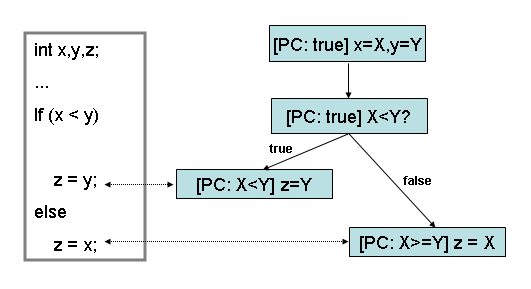
\includegraphics[scale=0.3]{symbolic}
		\end{figure}
		
		\begin{itemize}
			\item Symbolic values
			\item Path condition
			\item Limitations
			\begin{itemize}
				\item Path explosion
				\item Unbounded input
				\item Floating point values
			\end{itemize}
		\end{itemize}
	\end{frame}
	
	\begin{frame}
		\frametitle{Scheduling}
		
		\begin{figure}[htbp]
			\centering
			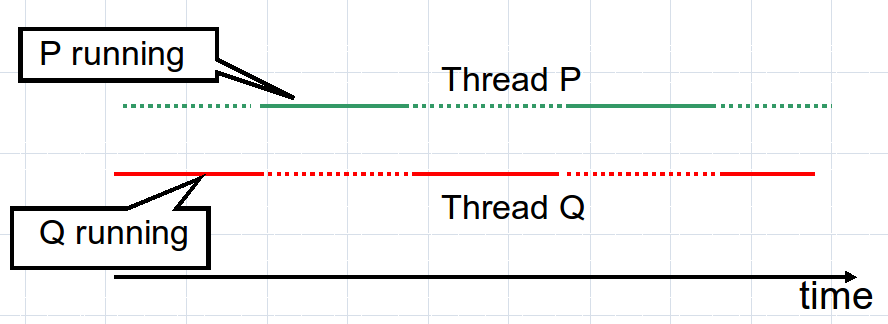
\includegraphics[scale=0.3]{interleaving}
		\end{figure}
		
		\begin{itemize}
			\item Thread interleaving
			\item Scheduler choices
			\begin{itemize}
				\item Thread wake-up
				\item Preemptions
			\end{itemize}
			\item Problems
			\begin{itemize}
				\item Path explosion when dealing with threads
			\end{itemize}
		\end{itemize}
	\end{frame}
	
	\begin{frame}
		\frametitle{Concolic testing}
		
		\begin{figure}[htbp]
			\centering
			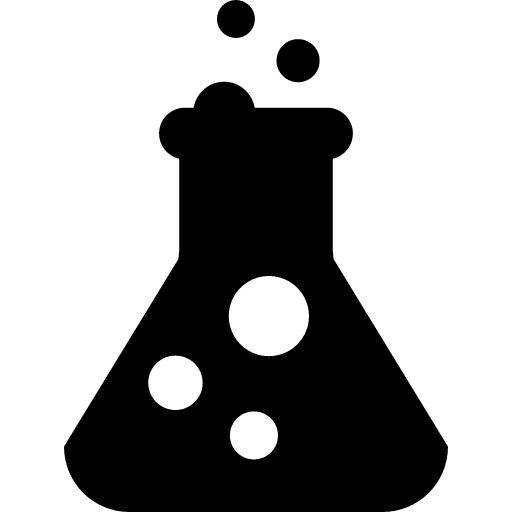
\includegraphics[scale=0.1]{concolic}
		\end{figure}
		
		\begin{itemize}
			\item Very practical approach
			\item Uses actual input to run a program
			\item Attempts to generate new input for further runs
			\item Problems
			\begin{itemize}
				\item Is not always complete (not all constraints can be solved)
				\item Finding inputs can be harder than standard symbolic execution
			\end{itemize}
			\item Advantages
			\begin{itemize}
				\item Faster
				\item Easy to generate tests
			\end{itemize}
		\end{itemize}
	\end{frame}
	
	\section{Approaches}
	
	%\subsection{Parallel Symbolic Execution for Automated Real-World Software Testing \cite{base3}}
	
	\setbeamercolor{frametitle}{fg=Paper1Full}
	
	\begin{frame}
		\frametitle{1. Parallel Symbolic Execution for Automated Real-World Software Testing \cite{base3} 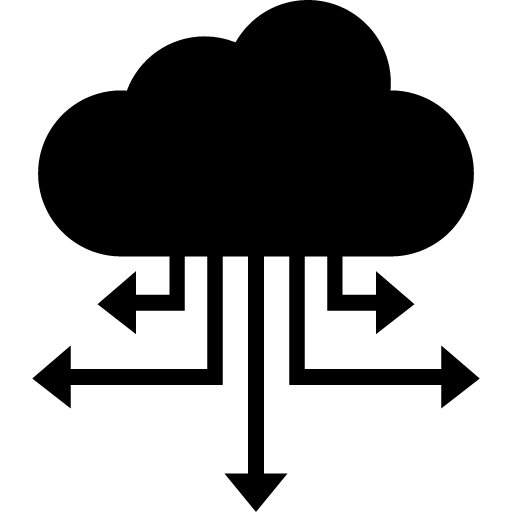
\includegraphics[scale=0.025]{distributed}}
		
		\begin{figure}[htbp]
			\centering
			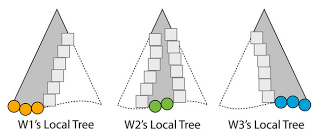
\includegraphics[scale=0.5]{cloud9}
		\end{figure}
		
		\begin{itemize}
			\item Method designed to test actual software
			\item Based on KLEE
			\begin{itemize}
				\item \url{https://klee.github.io/}
			\end{itemize}
			\item Extended POSIX support
			\begin{itemize}
				\item Standard API for applications
			\end{itemize}
			\item Distributed execution engine
			\item Simple to use
		\end{itemize}
	\end{frame}
	
	\begin{frame}
		\frametitle{Parallel Symbolic Execution for Automated Real-World Software Testing \cite{base3} 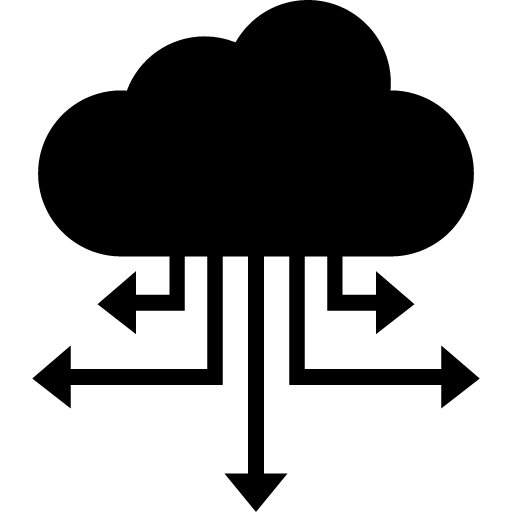
\includegraphics[scale=0.025]{distributed}}
		
		\begin{itemize}
			\item Not focused on concurrent software
			\item Depth of analysis can be selected for each test
			\begin{itemize}
				\item Complete analysis
				\item Iterative context bounding
				\item No preemption
				\item Deterministic scheduling (default)
			\end{itemize}
			\item Full POSIX threads support
		\end{itemize}
	\end{frame}
	
	\begin{frame}
		\frametitle{Iterative context bounding \cite{Musuvathi}}
		
		\begin{figure}[htbp]
			\centering
			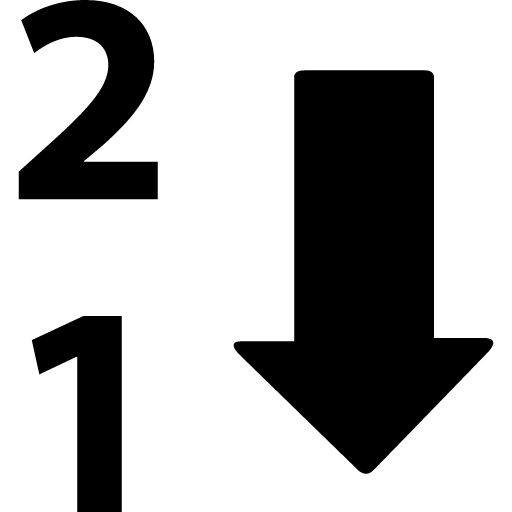
\includegraphics[scale=0.1]{limit}
		\end{figure}
		
		\begin{itemize}
			\item Simple search strategy
			\item Limits the number of preemptions
			\begin{itemize}
				\item Limit can be 0
				\item 90\% coverage using limit of 8
			\end{itemize}
			\item Normal execution is not affected
			\item Very likely to find most bugs
		\end{itemize}
	\end{frame}
	
	%\subsection{Concolic Testing of Multithreaded Programs and	Its Application to Testing Security Protocols \cite{base4}}
	\setbeamercolor{frametitle}{fg=Paper2Full}
	
	\begin{frame}
		\frametitle{2. Concolic Testing of Multithreaded Programs and	Its Application to Testing Security Protocols \cite{base4} 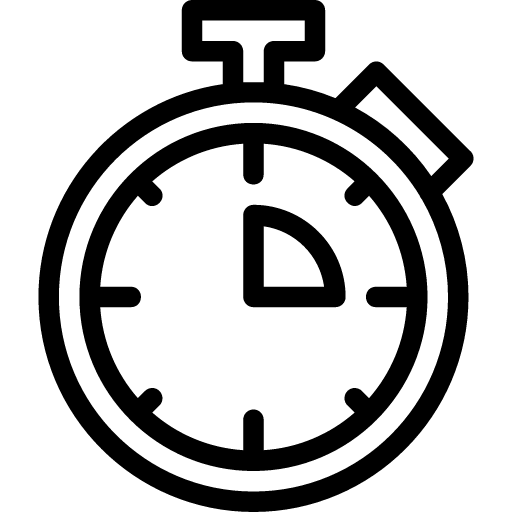
\includegraphics[scale=0.025]{clock}}
		
		\begin{itemize}
			\item Focused on reducing execution time of the analysis
			\item Implementation based on DVC
			\item Uses concolic testing for both input and scheduling
		\end{itemize}
	\end{frame}
	
	\begin{frame}
		\frametitle{Dynamic vector clocks (DVC) \cite{dvcproof}}
		
		\begin{figure}[htbp]
			\centering
			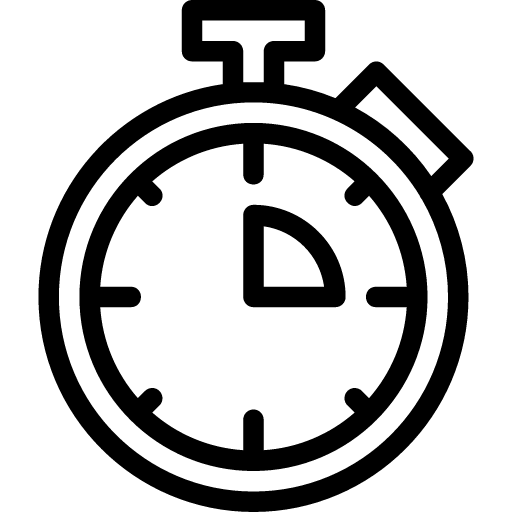
\includegraphics[scale=0.1]{clock}
		\end{figure}
		
		\begin{itemize}
			\item Detect possible race conditions
			\item Make analysis complete without the need to process all thread interleavings
			\item Easily computed during concolic execution
			\item Races can be flipped by postponing
		\end{itemize}
	\end{frame}

\defverbatim[colored]\lstI{
		\begin{lstlisting}[mathescape,tabsize=2,basicstyle=\tiny]
compute_next_input_and_schedule(input, path, branch_decisions)
	go trough the path backwards
		if you find a event
			if number of posponed threads < enabled threads
				if event has a race with a future event
					add current thread to postponed threads at the current event
					switch thread
					restart execution from the event
		else
			change branch_decision
			if $\exists$ input2 that satisfies branch_decision
				restart execution from the event
	no more executions found
		
		\end{lstlisting}
}
	
	
	\begin{frame}[fragile]
		\frametitle{Algorithm}

		\lstI
	\end{frame}
	
	%\subsection{Generalized Symbolic Execution for Model Checking and Testing \cite{base5}}
	\setbeamercolor{frametitle}{fg=Paper3Full}
	
	\begin{frame}
		\frametitle{3. Generalized Symbolic Execution for Model Checking and Testing \cite{base5} 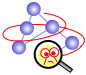
\includegraphics[scale=0.15]{jpf}}
		
		\begin{itemize}
			\item Can deal with \textbf{unbounded} input
			\item Uses Java PathFinder as a model checker
			\item Exhaustive search of all interleavings
		\end{itemize}
	\end{frame}
	
	\begin{frame}
		\frametitle{Generalized Symbolic Execution for Model Checking and Testing \cite{base5}}
		
		\begin{figure}[htbp]
			\centering
			%\includegraphics[bb=1.8in 6.5in 7.5in 9.5in,clip,page=3,scale=0.9]{GSE.pdf}
			\begin{tikzpicture}
			\node[anchor=south west,inner sep=0] at (0,0) {\includegraphics[bb=1.8in 6.5in 7.5in 9.5in,clip,page=3,scale=0.9]{GSE.pdf}};
			\fill[white] (0,5) rectangle (0.5,2);
			\node[draw] at (11.5,6) {1};
			\node[draw] at (11.5,5.3) {2};
			\node[draw] at (11.5,4.6) {3};
			\node[draw] at (11.5,2) {4};
			\end{tikzpicture}
		\end{figure}
	\end{frame}
	
	%\subsection{GKLEE: concolic verification and test generation for GPUs \cite{base7}}
	\setbeamercolor{frametitle}{fg=Paper4Full}
	
	\begin{frame}
		\frametitle{4. GKLEE: concolic verification and test generation for GPUs \cite{base7} 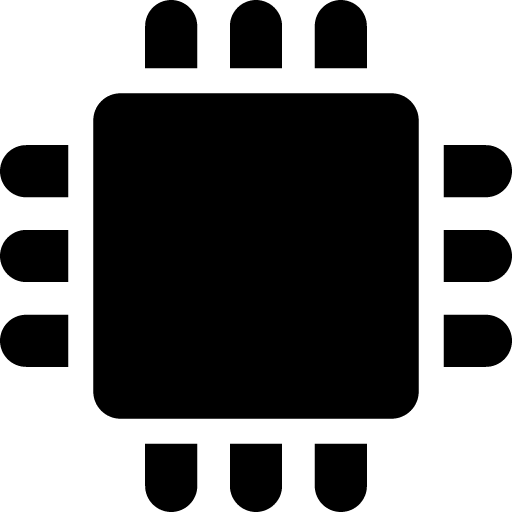
\includegraphics[scale=0.025]{gpu}}
		
		\begin{itemize}
			\item Specialized implementation for CUDA devices
			\begin{itemize}
				\item Compute Unified Device Architecture
				\item API + execution model
			\end{itemize}
			\item Scales very well to a very large number of threads
			\item Detects most concurrency errors and performance bottlenecks
		\end{itemize}
	\end{frame}
	
	\begin{frame}
		\begin{figure}[htbp]
			\centering
			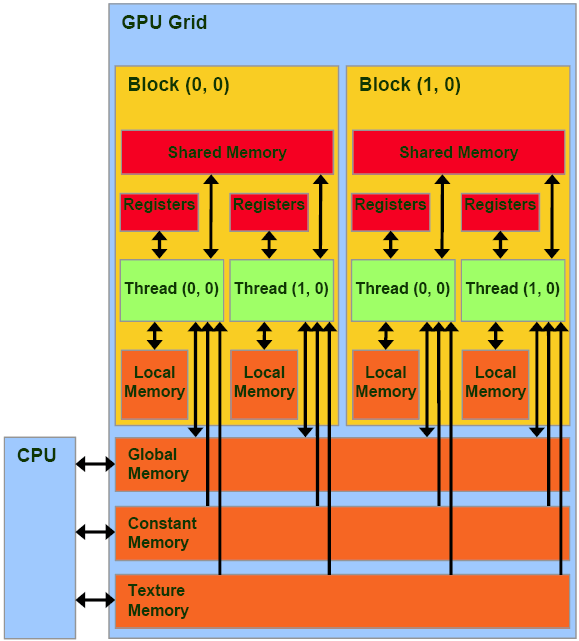
\includegraphics[scale=0.4]{CUDA-memory-model}
		\end{figure}
	\end{frame}
	
	\begin{frame}
		\frametitle{Approach}
		\begin{itemize}
			\item Takes advantage of hardware characteristics
			\begin{itemize}
				\item No preemptions
				\item SIMT (lockstep)
				\item Barriers are the only synchronization primitives
			\end{itemize}
			\item Results
			\begin{itemize}
				\item Deadlock
				\item Intra/Inter Race conditions
				\item Global races
				\item Access patterns
				\item Missing volatile
			\end{itemize}
		\end{itemize}
	\end{frame}
	
	\setbeamercolor{frametitle}{fg=Black}
	
	\section{Comparison}
	
	\begin{frame}
		\frametitle{Legend}
		
		\begin{itemize}
			\setbeamertemplate{itemize item}{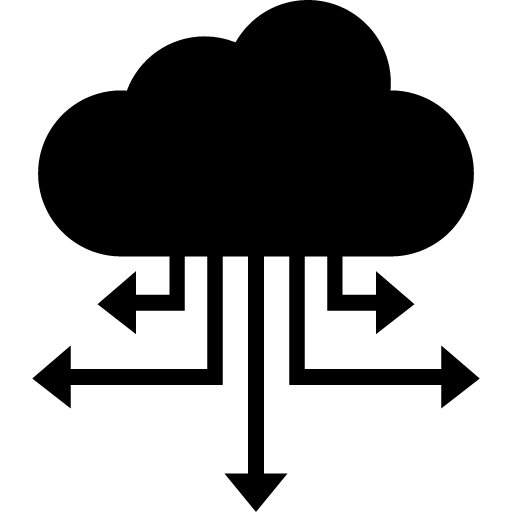
\includegraphics[scale=0.015]{distributed}}
			\color{Paper1Full} \setbeamercolor{item}{fg=Paper1Full} \item Parallel Symbolic Execution for Automated Real-World Software Testing
			\setbeamertemplate{itemize item}{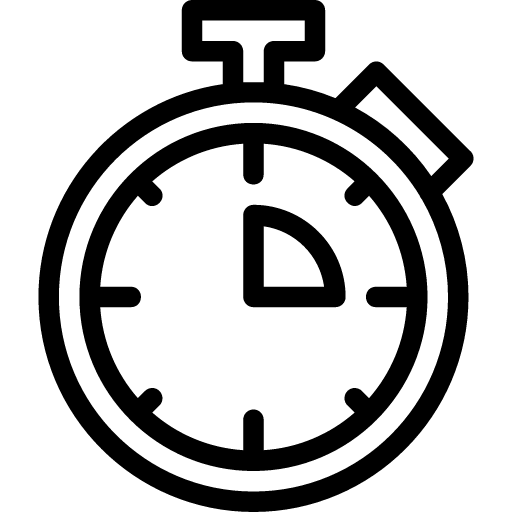
\includegraphics[scale=0.015]{clock}}
			\color{Paper2Full} \setbeamercolor{item}{fg=Paper2Full} \item Concolic Testing of Multithreaded Programs and	Its Application to Testing Security Protocols
			\setbeamertemplate{itemize item}{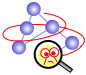
\includegraphics[scale=0.1]{jpf}}
			\color{Paper3Full} \setbeamercolor{item}{fg=Paper3Full} \item Generalized Symbolic Execution for Model Checking and Testing
			\setbeamertemplate{itemize item}{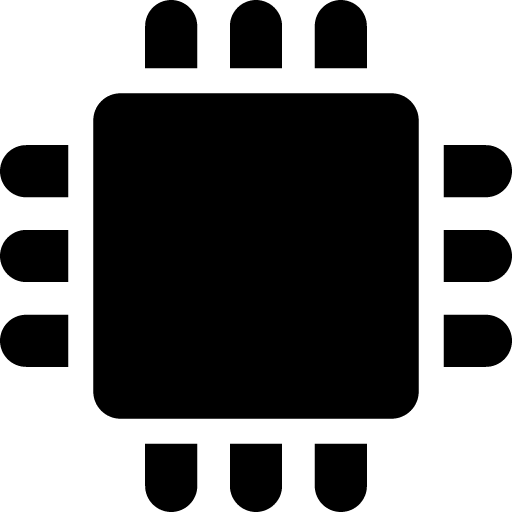
\includegraphics[scale=0.015]{gpu}}
			\color{Paper4Full} \setbeamercolor{item}{fg=Paper4Full} \item GKLEE: concolic verification and test generation for GPUs
		\end{itemize}
	\end{frame}
	
	\begin{frame}
		\frametitle{Comparison}
		
		\begin{tabular}{p{0.4\textwidth}p{0.5\textwidth}}
		
			Method
			\begin{itemize}
				\setbeamertemplate{itemize item}{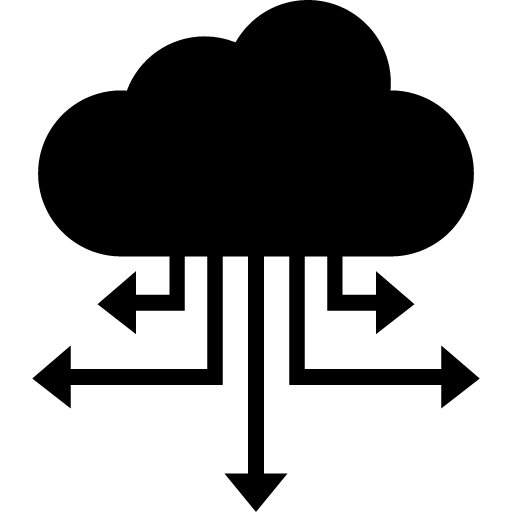
\includegraphics[scale=0.015]{distributed}}
				\color{Paper1Full} \setbeamercolor{item}{fg=Paper1Full} \item Concolic testing
				\setbeamertemplate{itemize item}{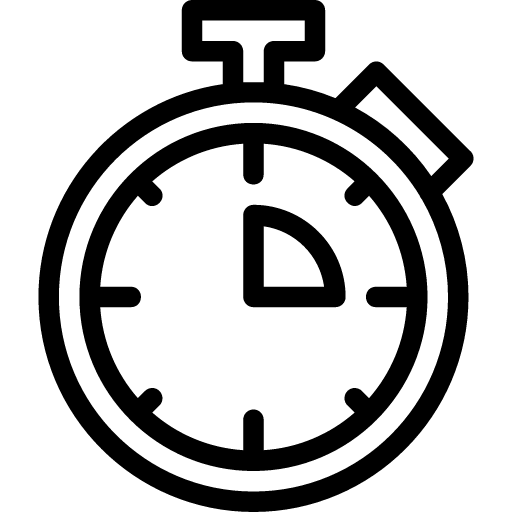
\includegraphics[scale=0.015]{clock}}
				\color{Paper2Full} \setbeamercolor{item}{fg=Paper2Full} \item Concolic testing
				\setbeamertemplate{itemize item}{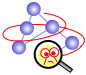
\includegraphics[scale=0.1]{jpf}}
				\color{Paper3Full} \setbeamercolor{item}{fg=Paper3Full} \item Model checking
				\setbeamertemplate{itemize item}{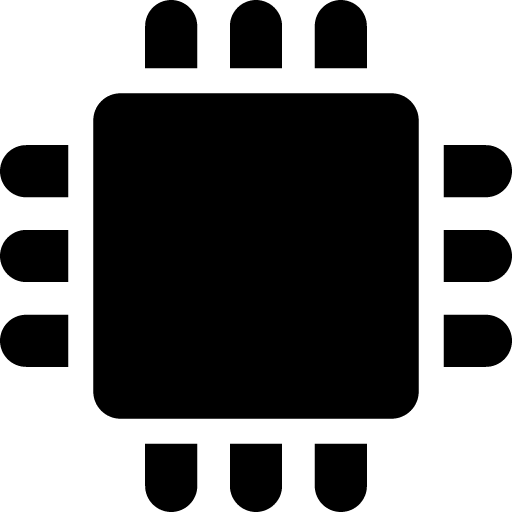
\includegraphics[scale=0.015]{gpu}}
				\color{Paper4Full} \setbeamercolor{item}{fg=Paper4Full} \item Concolic testing
			\end{itemize}
		&
			Automation/Required skill
			\begin{itemize}
				\setbeamertemplate{itemize item}{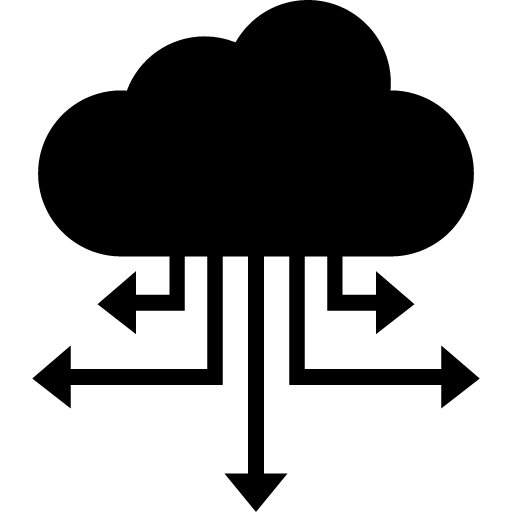
\includegraphics[scale=0.015]{distributed}}
				\color{Paper1Full} \setbeamercolor{item}{fg=Paper1Full} \item Full/Very low
				\setbeamertemplate{itemize item}{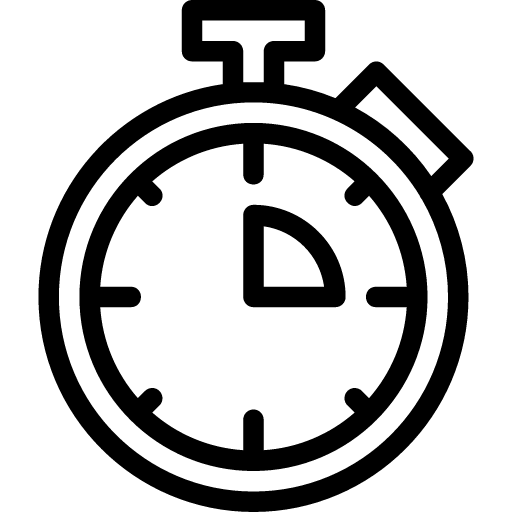
\includegraphics[scale=0.015]{clock}}
				\color{Paper2Full} \setbeamercolor{item}{fg=Paper2Full} \item Full/Low
				\setbeamertemplate{itemize item}{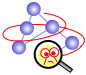
\includegraphics[scale=0.1]{jpf}}
				\color{Paper3Full} \setbeamercolor{item}{fg=Paper3Full} \item Full/Low
				\setbeamertemplate{itemize item}{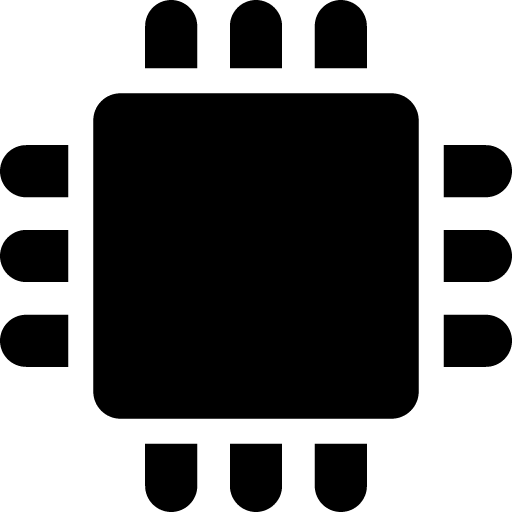
\includegraphics[scale=0.015]{gpu}}
				\color{Paper4Full} \setbeamercolor{item}{fg=Paper4Full} \item Full/Low
			\end{itemize}	
		\\
			Applicability
			\begin{itemize}
				\setbeamertemplate{itemize item}{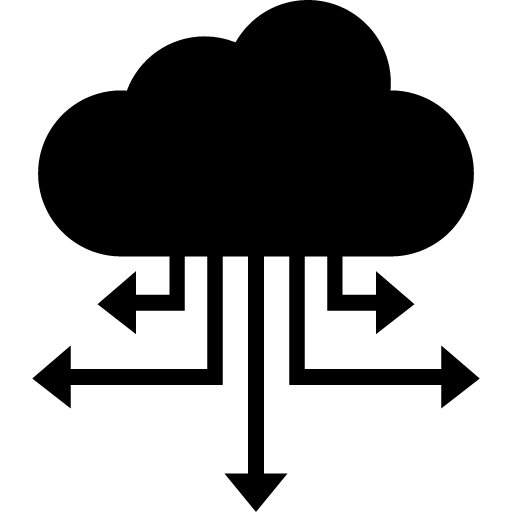
\includegraphics[scale=0.015]{distributed}}
				\color{Paper1Full} \setbeamercolor{item}{fg=Paper1Full} \item POSIX
				\setbeamertemplate{itemize item}{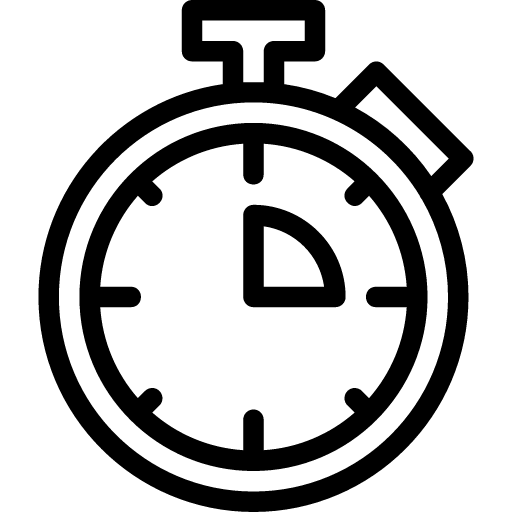
\includegraphics[scale=0.015]{clock}}
				\color{Paper2Full} \setbeamercolor{item}{fg=Paper2Full} \item Java
				\setbeamertemplate{itemize item}{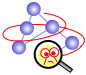
\includegraphics[scale=0.1]{jpf}}
				\color{Paper3Full} \setbeamercolor{item}{fg=Paper3Full} \item Java
				\setbeamertemplate{itemize item}{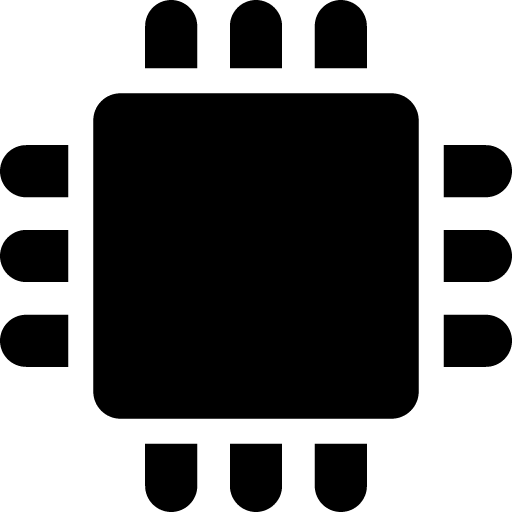
\includegraphics[scale=0.015]{gpu}}
				\color{Paper4Full} \setbeamercolor{item}{fg=Paper4Full} \item CUDA
			\end{itemize}
		&
			Goal
			\begin{itemize}
				\setbeamertemplate{itemize item}{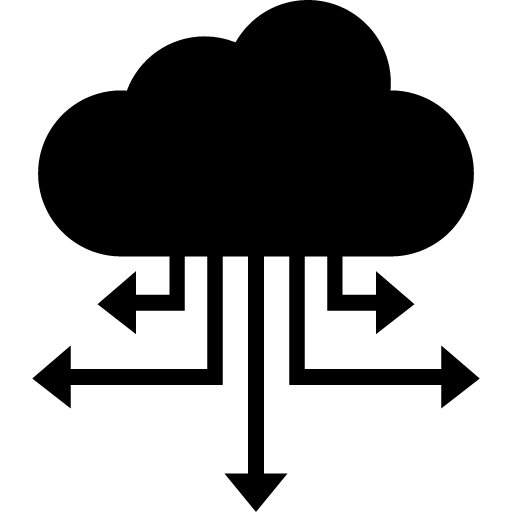
\includegraphics[scale=0.015]{distributed}}
				\color{Paper1Full} \setbeamercolor{item}{fg=Paper1Full} \item Testing
				\setbeamertemplate{itemize item}{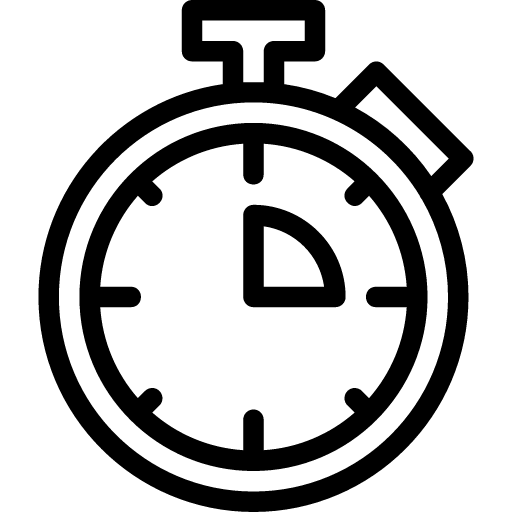
\includegraphics[scale=0.015]{clock}}
				\color{Paper2Full} \setbeamercolor{item}{fg=Paper2Full} \item Testing
				\setbeamertemplate{itemize item}{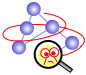
\includegraphics[scale=0.1]{jpf}}
				\color{Paper3Full} \setbeamercolor{item}{fg=Paper3Full} \item Testing
				\setbeamertemplate{itemize item}{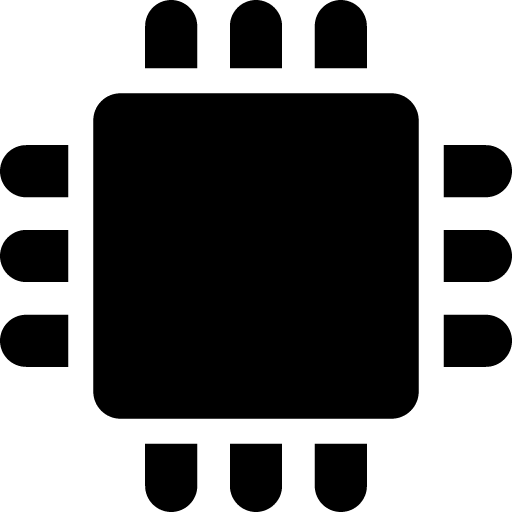
\includegraphics[scale=0.015]{gpu}}
				\color{Paper4Full} \setbeamercolor{item}{fg=Paper4Full} \item Testing + Performance bottlenecks
			\end{itemize}
		\end{tabular}
	\end{frame}
	
	\begin{frame}
		\frametitle{Concurrency}
		
		\begin{tabular}{p{0.4\textwidth}p{0.5\textwidth}}
			
			Performance/threads
			\begin{itemize}
				\setbeamertemplate{itemize item}{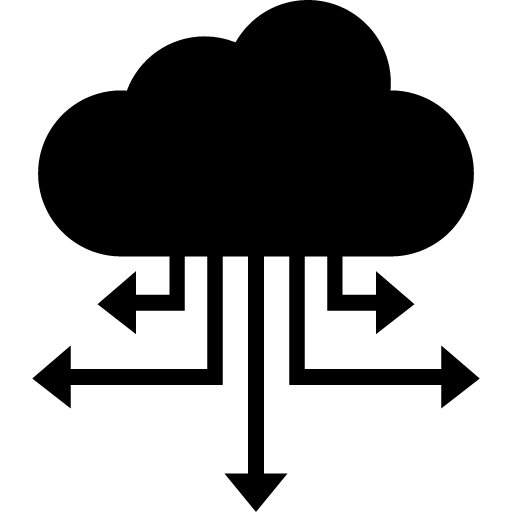
\includegraphics[scale=0.015]{distributed}}
				\color{Paper1Full} \setbeamercolor{item}{fg=Paper1Full} \item Low, brute force available
				\setbeamertemplate{itemize item}{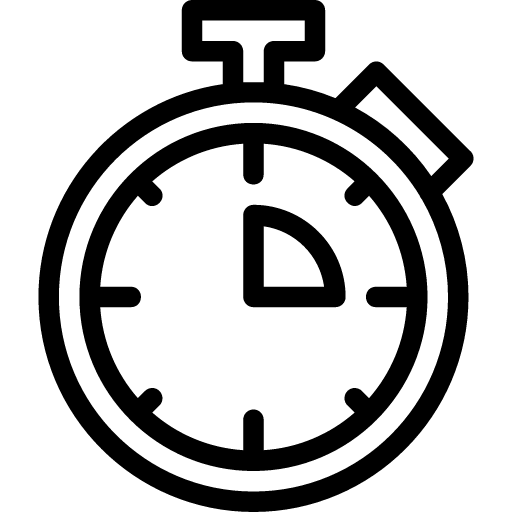
\includegraphics[scale=0.015]{clock}}
				\color{Paper2Full} \setbeamercolor{item}{fg=Paper2Full} \item Medium
				\setbeamertemplate{itemize item}{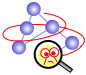
\includegraphics[scale=0.1]{jpf}}
				\color{Paper3Full} \setbeamercolor{item}{fg=Paper3Full} \item Low
				\setbeamertemplate{itemize item}{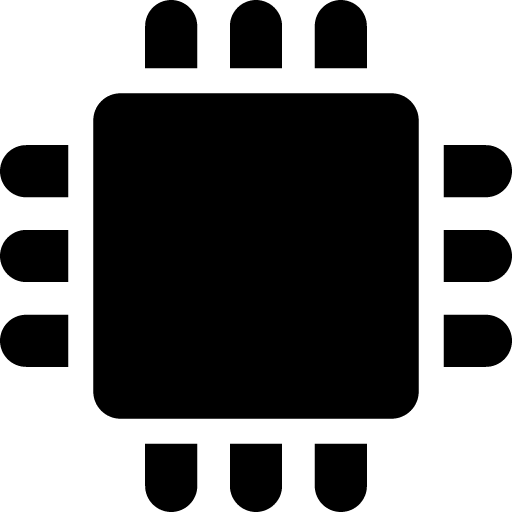
\includegraphics[scale=0.015]{gpu}}
				\color{Paper4Full} \setbeamercolor{item}{fg=Paper4Full} \item Very good
			\end{itemize}
			&
			Performance/input size
			\begin{itemize}
				\setbeamertemplate{itemize item}{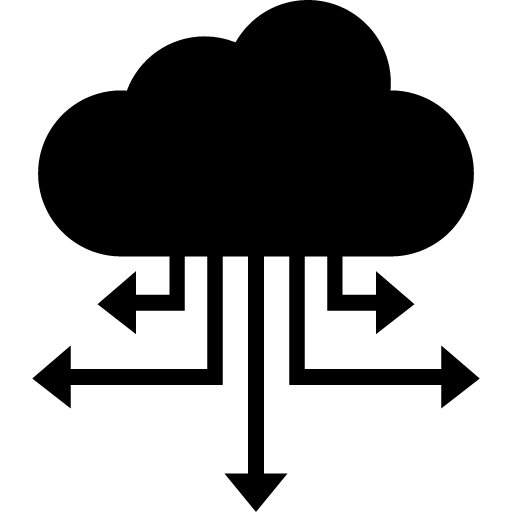
\includegraphics[scale=0.015]{distributed}}
				\color{Paper1Full} \setbeamercolor{item}{fg=Paper1Full} \item Low, brute force available
				\setbeamertemplate{itemize item}{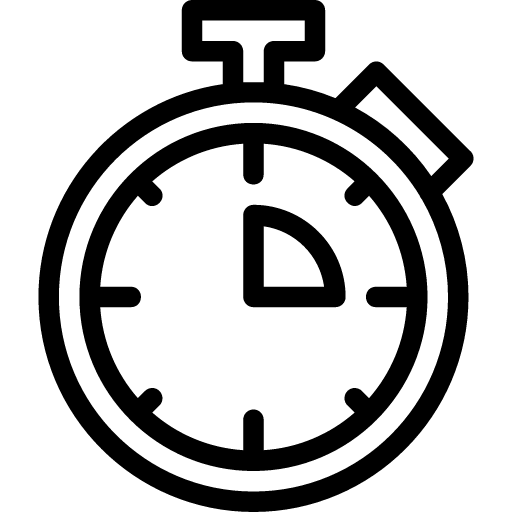
\includegraphics[scale=0.015]{clock}}
				\color{Paper2Full} \setbeamercolor{item}{fg=Paper2Full} \item Low
				\setbeamertemplate{itemize item}{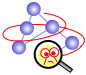
\includegraphics[scale=0.1]{jpf}}
				\color{Paper3Full} \setbeamercolor{item}{fg=Paper3Full} \item Low
				\setbeamertemplate{itemize item}{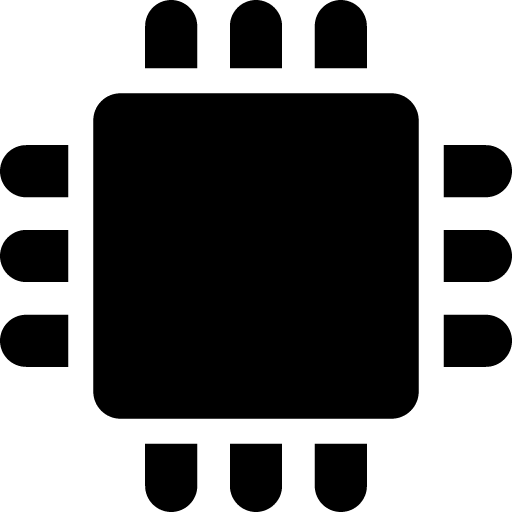
\includegraphics[scale=0.015]{gpu}}
				\color{Paper4Full} \setbeamercolor{item}{fg=Paper4Full} \item Good
			\end{itemize}	
			\\
			Complete analysis
			\begin{itemize}
				\setbeamertemplate{itemize item}{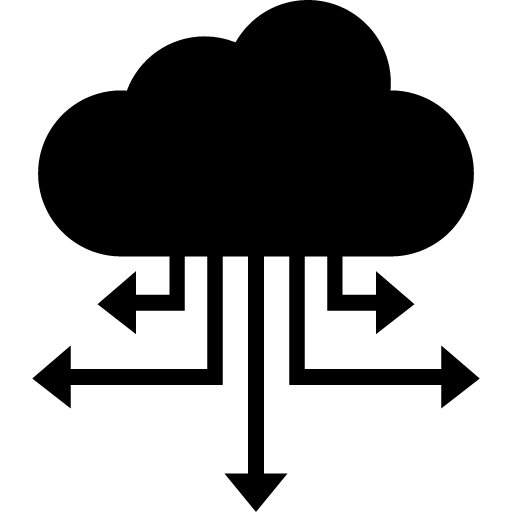
\includegraphics[scale=0.015]{distributed}}
				\color{Paper1Full} \setbeamercolor{item}{fg=Paper1Full} \item Optional
				\setbeamertemplate{itemize item}{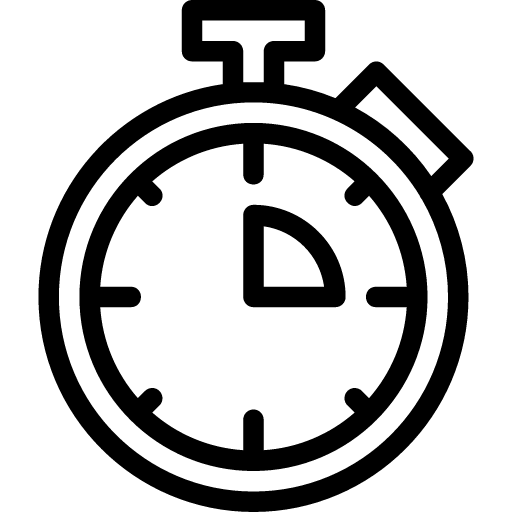
\includegraphics[scale=0.015]{clock}}
				\color{Paper2Full} \setbeamercolor{item}{fg=Paper2Full} \item Unlikely
				\setbeamertemplate{itemize item}{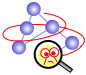
\includegraphics[scale=0.1]{jpf}}
				\color{Paper3Full} \setbeamercolor{item}{fg=Paper3Full} \item Yes
				\setbeamertemplate{itemize item}{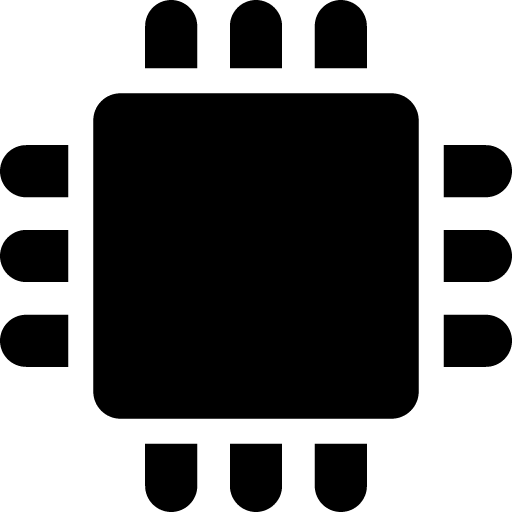
\includegraphics[scale=0.015]{gpu}}
				\color{Paper4Full} \setbeamercolor{item}{fg=Paper4Full} \item Yes
			\end{itemize}
			&
			Partial results
			\begin{itemize}
				\setbeamertemplate{itemize item}{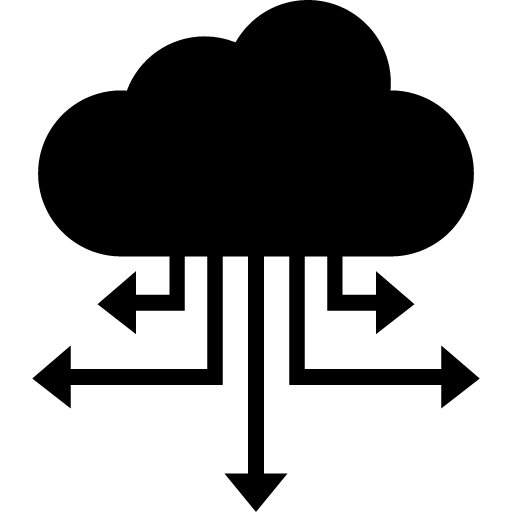
\includegraphics[scale=0.015]{distributed}}
				\color{Paper1Full} \setbeamercolor{item}{fg=Paper1Full} \item Yes
				\setbeamertemplate{itemize item}{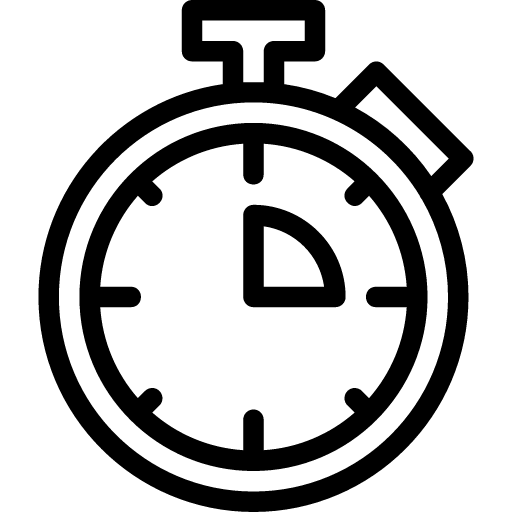
\includegraphics[scale=0.015]{clock}}
				\color{Paper2Full} \setbeamercolor{item}{fg=Paper2Full} \item Yes
				\setbeamertemplate{itemize item}{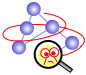
\includegraphics[scale=0.1]{jpf}}
				\color{Paper3Full} \setbeamercolor{item}{fg=Paper3Full} \item No
				\setbeamertemplate{itemize item}{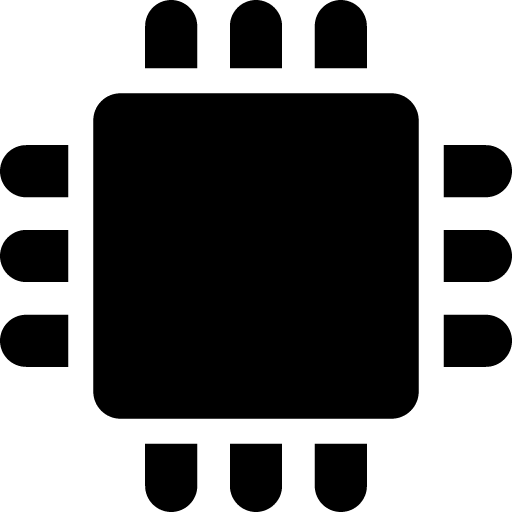
\includegraphics[scale=0.015]{gpu}}
				\color{Paper4Full} \setbeamercolor{item}{fg=Paper4Full} \item No
			\end{itemize}
		\end{tabular}
		
		
	\end{frame}
	
	\section{Conclusions}
	
	\begin{frame}
		\frametitle{Conclusions}
		
		\begin{itemize}
			\item Many developments
			\item No one best approach, but most methods can be combined
			\item Hopefully more research in the field
		\end{itemize}
	\end{frame}
	
	\begin{frame}
		Questions
	\end{frame}
	
	%\section{References}
	
	\begin{frame}
		\frametitle{References}
		\tiny
		\bibliographystyle{splncs03}
		\bibliography{ref}
	\end{frame}
\end{document}
